\documentclass{standalone}

\usepackage{tikz}
\usepackage{pgfplots}

\usetikzlibrary{calc}

\begin{document}
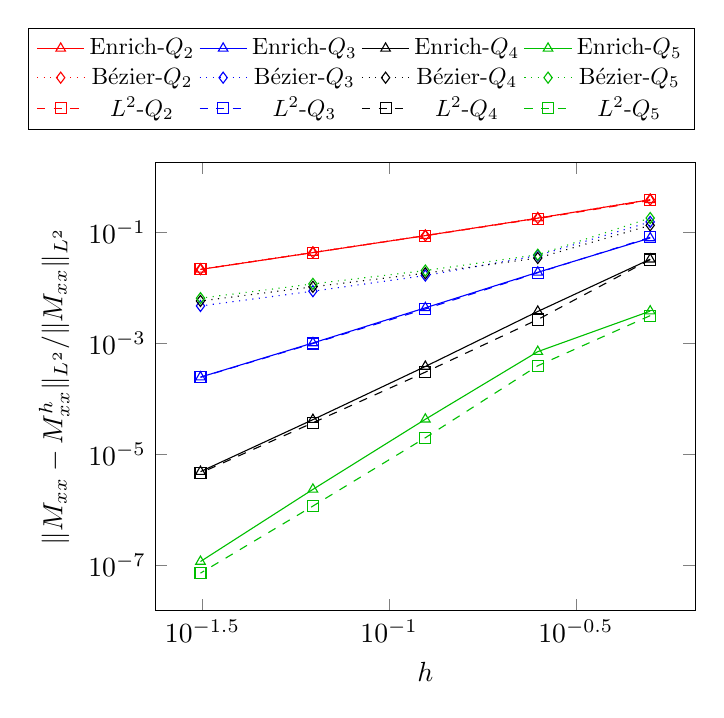
\begin{tikzpicture}
    \begin{loglogaxis}[
        legend columns=4,
    	legend style={at={(1,1.3)}, nodes={scale=.85, transform shape}},
        xlabel=$h$,
        ylabel=${\|M_{xx}-M_{xx}^{h}\|_{L^2}}/{\|M_{xx}\|_{L^2}}$ 
    ]

    \addplot [color=red,mark=triangle] plot coordinates {

        (.5,        0.388683)
        (.25,       0.180344)
        (.125,      0.0873936)
        (.0625,     0.0431786)
        (0.03125,   0.0214827)
    };

    
    \addplot [color=blue,mark=triangle] plot coordinates {

        (.5,        0.0791641)
        (.25,       0.0190616)
        (.125,      0.00436081)
        (.0625,     0.00101346)
        (0.03125,   0.000245449)
    };

    \addplot [color=black,mark=triangle] plot coordinates {

        (.5,        0.0328205)
        (.25,       0.00375056)
        (.125,      0.00038177)
        (.0625,     4.19797e-05)
        (0.03125,   4.84872e-06)
    };

    \addplot [color=green!75!black,mark=triangle] plot coordinates {


        (.5,        0.00380016)
        (.25,       0.000707366)
        (.125,      4.26557e-05)
        (.0625,     2.32106e-06)
        (0.03125,   1.16179e-07)
    };

    
    \addplot [color=red,mark=diamond, every mark/.append style={solid}, dotted] plot coordinates {

        (.5,        0.391114)
        (.25,       0.181228)
        (.125,      0.088122)
        (.0625,     0.0436043)
        (0.03125,   0.0217303)
    };

    
    \addplot [color=blue,mark=diamond, every mark/.append style={solid}, dotted] plot coordinates {

        (.5,        0.154476)
        (.25,       0.0382179)
        (.125,      0.0166483)
        (.0625,     0.00870388)
        (0.03125,   0.0047146)
    };

    \addplot [color=black,mark=diamond, every mark/.append style={solid}, dotted] plot coordinates {


        (.5,        0.133896)
        (.25,       0.0344995)
        (.125,      0.018339)
        (.0625,     0.0104405)
        (0.03125,   0.00579694)
    };

    \addplot [color=green!75!black,mark=diamond, every mark/.append style={solid}, dotted] plot coordinates {

        (.5,        0.181391)
        (.25,       0.0395733)
        (.125,      0.0204977)
        (.0625,     0.0117788)
        (0.03125,   0.00650763)
    };


    \addplot [color=red,mark=square, every mark/.append style={solid}, dashed] plot coordinates {

        (.5,        0.377159)
        (.25,       0.177245)
        (.125,      0.0871317)
        (.0625,     0.0431889)
        (0.03125,   0.0214911)
    };

    
    \addplot [color=blue,mark=square, every mark/.append style={solid}, dashed] plot coordinates {

        (.5,        0.081315)
        (.25,       0.018738)
        (.125,      0.00415793)
        (.0625,     0.00099096)
        (0.03125,   0.000243399)
    };

    \addplot [color=black,mark=square, every mark/.append style={solid}, dashed] plot coordinates {

        (.5,        0.0323516)
        (.25,       0.00268255)
        (.125,      0.000302014)
        (.0625,     3.68635e-05)
        (0.03125,   4.59608e-06)
    };

    \addplot [color=green!75!black,mark=square, every mark/.append style={solid}, dashed] plot coordinates {

        (.5,        0.00314999)
        (.25,       0.000393817)
        (.125,      1.9796e-05)
        (.0625,     1.16125e-06)
        (0.03125,   7.16873e-08)
    };


    \logLogSlopeTriangle{0.16}{0.075}{0.06}{4}{green!75!black};
    \logLogSlopeTriangle{0.16}{0.075}{0.28}{3}{black};
    \logLogSlopeTriangle{0.16}{0.075}{0.495}{2}{blue};
    \logLogSlopeTriangle{0.16}{0.075}{0.74}{1}{red};

    \legend{Enrich-$Q_2$\\Enrich-$Q_3$\\Enrich-$Q_4$\\Enrich-$Q_5$\\B\'ezier-$Q_2$\\B\'ezier-$Q_3$\\B\'ezier-$Q_4$\\B\'ezier-$Q_5$\\$L^2$-$Q_2$\\$L^2$-$Q_3$\\$L^2$-$Q_4$\\$L^2$-$Q_5$\\}
    \end{loglogaxis}
\end{tikzpicture}

\end{document}
